\chapter{Lösungsdesign}

Das Lösungsdesign beinhaltet die Grundlagen für die erfolgreiche Umsetzung des Prototypen. Basierend auf den Anforderungen und der Aufgabenstellung wird die Software-Architektur definiert. Wäh\-rend dies auf einer hohen Abstraktionsebene geschieht, erfolgt in einem nächsten Schritt der Entwurf und das Design der Software. Dabei dient die Architektur als Leitplanke, welche zusammen mit der Recherche über den aktuellen Stand der Technik (\autoref{literatur}) zu einem konkreten Entwurf führen.

\section{Architektur}\label{architecture}

Der Architektur-Entwurf betrachtet die zu entwickelnde Software aus einer abstrakten Sicht, wobei die tatsächliche verwendete Software, keinen Einfluss hat. Das Ziel ist eine grundsätzliche Übersicht über die Software, deren Komponenten, Schnittstellen und auch deren Verteilung.


Basierend auf den Anforderungen (\autoref{sec:anforderungen}) an den zu entwickelnden Prototypen, wird im folgenden Abschnitt die zugrundeliegende Architektur-Entwurf ausgeführt. Die Ar\-chi\-tek\-tur-\-Ent\-schei\-dung\-en bilden die Grundlage für die Designentscheidungen für den Soft\-wa\-re-\-Ent\-wurf. Grundlegend orientieren wir uns bei dem Entwurf an dem \textit{4+1 Schichtenmodell}. \\\cite{kruchten1995architectural}.


%\url{https://www4.in.tum.de/misc/perlen/perlen-folien/PDW_Architektur_IK_Druckversion.pdf}\\
%\url{http://www.edv-buchversand.de/chapter.php?cnt=getchapter&id=ha-41215_2.pdf}\\


\subsection{Kontextsicht}
    \begin{figure}[ht]
    \centering
    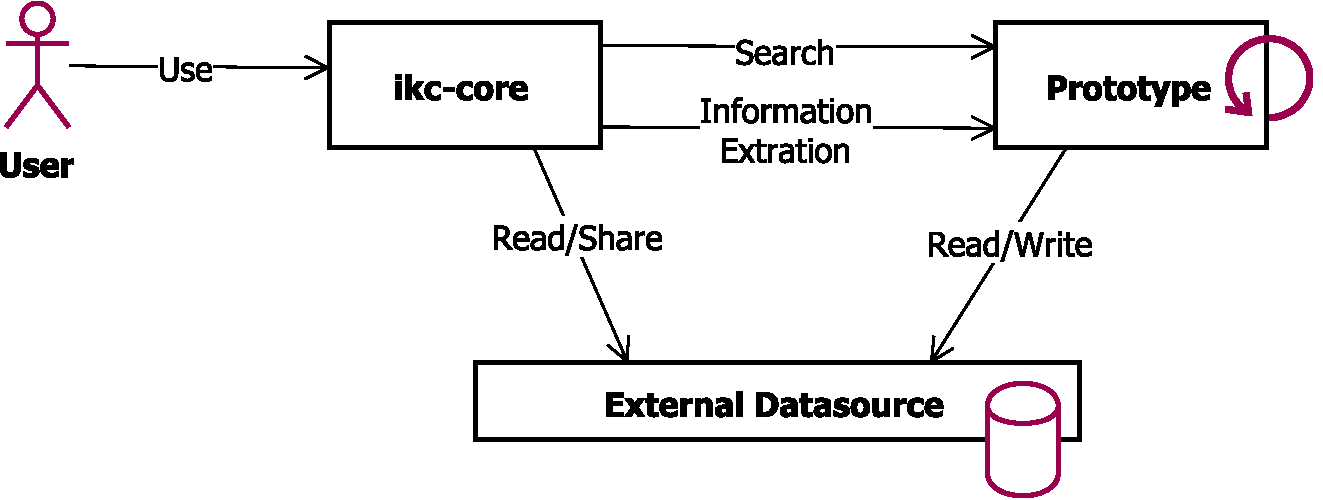
\includegraphics[width=1\textwidth]{BDA_Context}
    \caption{Kontextsicht}
    \label{fig:kontextsicht}
    \end{figure}
 
 Die \autoref{fig:kontextsicht} gibt einen Überblick über den Kontext des zu entwickelnden Prototypen:
 Der \texttt{ikc-core} nutzt den Prototypen zur Erweiterung seiner Funktionalität. Damit können die Hauptanforderungen, die Volltextsuche und die Extraktion von Schlüsselwörter, abgedeckt werden. Diese beiden Funktionen sind für den Benutzer über das \texttt{UserInterface} innerhalb des \gls{ikc-core} verfügbar. Sowohl der \gls{ikc-core} als auch der Prototyp haben Zugriff auf die externen Datenquelle. Der Prototyp hat dort die Quellen für die Dateiinhalte und hält dort auch Indizes für die Volltextsuche und die Schlü\-ssel\-wort-Ex\-trak\-tion.
 



\subsection{Einflussfaktoren}\label{einflussfaktoren}

Basierend auf dem Kontext des \gls{ikc-core}, dem Scope und der funktionalen und nichtfunktionalen Anforderungen beeinflussen verschiedenen Faktoren den Architektur Entwurf.

\begin{longtable}{|p{4cm}|p{8.5cm}|}

  \hline
    Faktor &  Beschreibung \\\hline
    Browseranwendung & Der \gls{ikc-core} ist als clientseitige Browseranwendung aufgebaut und kann bis anhin grundsätzlich ohne serverseitige Logik genutzt werden. %Funktionale Erweiterungen mit Hilfe von zusätzlicher zentralen Services sind in Entwicklung. Diese betreffen jedoch keine grundlegenden Funktionen der Applikation.
    \\\hline
    Mehrplatz-Nutzung & Soll der \gls{ikc-core} in einer Mehrplatz-Umgebung genutzt werden, ist eine Synchronisation auf \gls{Dropbox} notwendig. Diese muss vom Benutzer explizit angegeben und authorisiert werden.\\\hline
    Hardware Infrastruktur & Die Server-Infrastruktur des Departements Informatik (\textit{enterpriselab}) bietet die Ressourcen, auf welchen die Webanwendung läuft. Dazu werden zwei virtuelle \gls{Ubuntu}-Server verwendet. Die Entwicklung und die Produktion sind somit komplett voneinander getrennt.\\\hline
    
    Software Infrastruktur & Als Basis für Applikationsverteilung auf die Entwicklungs- und Produktions-System wird \gls{Dokku} in Kombination mit \gls{Gitlab CI} verwendet. Änderungen so direkt aus dem Versionskontrollsystem verteilt. Die Software wird als \gls{Docker}-Container ausgeliefert und anschliessend als dedizierte Applikation innerhalb des \gls{Dokku}-Frameworks gestartet.\\\hline
    
    Programmiersprachen & Als Programmiersprache wird \gls{Typescript} verwendet. Anders als andere Webprogrammiersprachen wie \gls{Javascript} ermöglicht sie die Verwendung von Sprachkonstrukten der Typisierung, wie zum Beispiel Klassen oder Vererbung. Durch den Typescript-Kompiler wird der Code für die Ausführung in reinen \gls{Javascript} Code übersetzt. Mit der Verwendung der \gls{Node}-Plattform kann \gls{Typescript} auch für eine Server Anwendung verwendet werden. Dadurch steigt sowohl die Wiederverwendbarkeit als Skalierbarkeit.\\\hline
    
    Kommunikation & Für eine allfällige Kommunikation zwischen dem \gls{ikc-core} und einer serverseitigen Erweiterung wird über einen Websocket abgehandelt. Dadurch wird eine beidseitige Kommunikation ermöglicht. \\\hline
    
    UI-Framework & Die Verwendung des \gls{React}-Frameworks ermöglicht den modularen Aufbau des \texttt{ikc-core}. Die gesamte Oberfläche ist in verschiedene Elemente aufgeteilt, welche über den Applikationzustand gesteuert werden. Eingaben des Benutzers werden durch die verschiedenen \texttt{UI Services} abgearbeitet und resultieren in einem aktualisierten Applikationszustand. Der unidirektionale Datenfluss sorgt für die klare Trennung der Verantwortlichkeiten innerhalb der \texttt{UI Services}. \\\hline
    
    Datenhaltung & Der \gls{ikc-core} nutzt keine zentralen Services für die Persistenz von den Daten der Benutzer oder deren Applikations-Konfiguration. Es werden die lokalen Ressourcen oder externe Datenquellen wie \gls{Dropbox} verwendet. \\\hline
    \caption{Einflussfaktoren}
  \label{tab:einflussfaktoren}
\end{longtable}


%Der \gls{ikc-core} ist primär eine Browserapplikation, der Grossteil der verwendeten Komponenten läuft ebenfalls clientseitig. Die Kommunikation mit serverseitigen Services funktioniert über REST-Schnittstellen oder WebSockets. Darunter gehört beispielsweise eine Schnittstelle mit \gls{Evernote}. Dies hat insbesondere den Grund, dass durch die Nutzung des \gls{ikc-core} keine zusätzliche Persistenz eingeführt wird. Darum sind keine zentralen Applikations- und Datenserver notwendig.

%Dies schränkt die Architektur insoweit ein, dass Komponenten mit kritischer Funktionalität oder Leistung möglichst gekapselt und entkoppelt sind. Nur in diesem Fall ist gewährleistet, dass eine entsprechende Komponente, falls notwendig, auch auf einer Server-\-Um\-geb\-ung laufen kann.

\subsection{Architekturtreiber}
Zwei elementare Architekturtreiber beeinflussen die Konzeption des Prototyps. Diese wurden bereits weiter oben als Einflussfaktor (\autoref{einflussfaktoren}) erwähnt, haben jedoch auch für den Prototyp eine zentrale Bedeutung.

\begin{itemize}
    \item \textbf{Entkopplung und Wiederverwendbarkeit}:
    Module und Komponenten sind entkoppelt voneinander. Dadurch können diese innerhalb der Applikation, oder auch für zukünftige Projekte, leicht wiederverwendet werden. Bei Performance-Engpässen ist es weiter möglich, bestimmte Module auszulagern, dies sowohl lokal innerhalb der Client-Applikation, als auch extern auf eine Server-Umgebung.
    \item \textbf{Verhinderung von zusätzlicher Persistenz}:
    Applikationsdaten- und Konfiguration sind stets lediglich von den bestehenden Datenquellen zu beziehen. Hierbei handelt es sich entweder um den lokalen Cache des Benutzers oder die entsprechende externe Datenquelle. Durch diesen Umstand kann viel Zeit für die Entwicklung und die Absicherung einer Persistenz-Infrastruktur gespart werden. Der Benutzer hat so zusätzlich immer eine transparente Kontrolle über den Speicherort und auch den Inhalt der eigenen Daten.
    \item \textbf{Inspiration durch React und Flux}: Wie in \autoref{react} bereits erwähnt, arbeitet React im Hintergrund mit einer eigenen Implementation von Flux. Dieser orientiert sich stark am funktionalen Programmier-Paradigma: Innere Zustände, also Variabeln, sind wann immer möglich zu verhindern. Dies wirkt allfälligen Seiteneffekten entgegen, macht den Code so nachvollziehbarer. Auch der unidirektionale Datenfluss strebt ähn\-liche Ziele an. Diese Überlegungen begleiteten die Entwicklung ständig. So sind an vielen Orten Programmierkonstrukte zu finden, welche prinzipiell verwandte Ansätze verfolgen.
\end{itemize}

\subsection{Architekturziele}

Der zu entwickelnde Prototyp baut auf dem bestehenden \gls{ikc-core} auf. Dabei soll das Augenmerk weiterhin auf den bereits bestehenden Eigenschaften der Architektur, insbesondere der Modularität und der Erweiterbarkeit, gehalten werden. Dies ist im Kontext des zugrundeliegenden Forschungsprojekts von hoher Wichtigkeit. Die Vergangenheit hat gezeigt, dass eine solide aber gleichzeitig auch anpassungsfähige Basis ein kritischer Faktor für die agile Weiterentwicklung ist. Einzig unter diesen Voraussetzungen ist es möglich auf die stetig ändernden Anforderungen entsprechend zu reagieren.

Die wichtigsten Ziele der Architektur sind in folgender Tabelle (\autoref{tab:architekturziele}) kurz erläutert:

\begin{longtable}{|p{4.5cm}|p{8.5cm}|}

  \hline
    Ziel &  Beschreibung \\\hline
    Modularität & Die verschiedenen Komponenten sind auswechselbar und an anderen Orten wiederverwendbar. Eine lose Kopplung und eine hohe Kohäsion innerhalb der Komponenten und deren Klassen ist dafür vorausgesetzt.\\\hline
    Erweiterbarkeit & Die Komponenten sind offen für Erweiterungen. Ein Ausbau der Funktionalität ist stets möglich.\\\hline
    Skalierbarkeit & Durch Bildung von Schichten ist es möglich einzelne Komponenten horizontal zu skalieren. Das bedeutet, dass mehrere gleiche Services beispielsweise sich einzelne Aufgaben teilen können. Dafür sind diverse Szenarien denkbar. Die Performance kann so an bestimmten Stellen optimiert werden.\\\hline
%    Vorbereitung Multiuser-Betrieb & \\\hline
    Benutzerfreundlichkeit & Bezüglich der Benutzeroberfläche ist es wichtig, dass der Benutzer immer über die Abläufe im Hintergrund informiert wird. Insbesondere bei der aufwändigen Verarbeitung von grossen Datenmengen, ist er Benutzer nie gehindert oder gar blockiert seine Arbeit mit dem Prototypen fortzusetzen. Sind die Resultate verfügbar, wird er benachrichtigt und kann auf deren Basis weiterarbeiten.\\\hline
    Performance & \\\hline
    \caption{Ziele der Architektur}
  \label{tab:architekturziele}
\end{longtable}

% Performance, Stresstest, Flexibilität, Erweiterbarkeit, Benutzerfreundlichkeit
% anderer Kontext, ...
%Entkoppelt, einfach erweiterbar, modularisiert, microservices, skalierbar


\subsection{Bausteinsicht}
Die \autoref{fig:bausteinsicht} beschreibt die Bausteinsicht der Architektur des Prototypen. Darin werden die verschiedenen Komponenten und Module und deren Beziehungen untereinander aufgezeigt. Hierbei werden drei verschiedene Abstraktionslevel unterschieden. 

\begin{figure}[H]
\centering
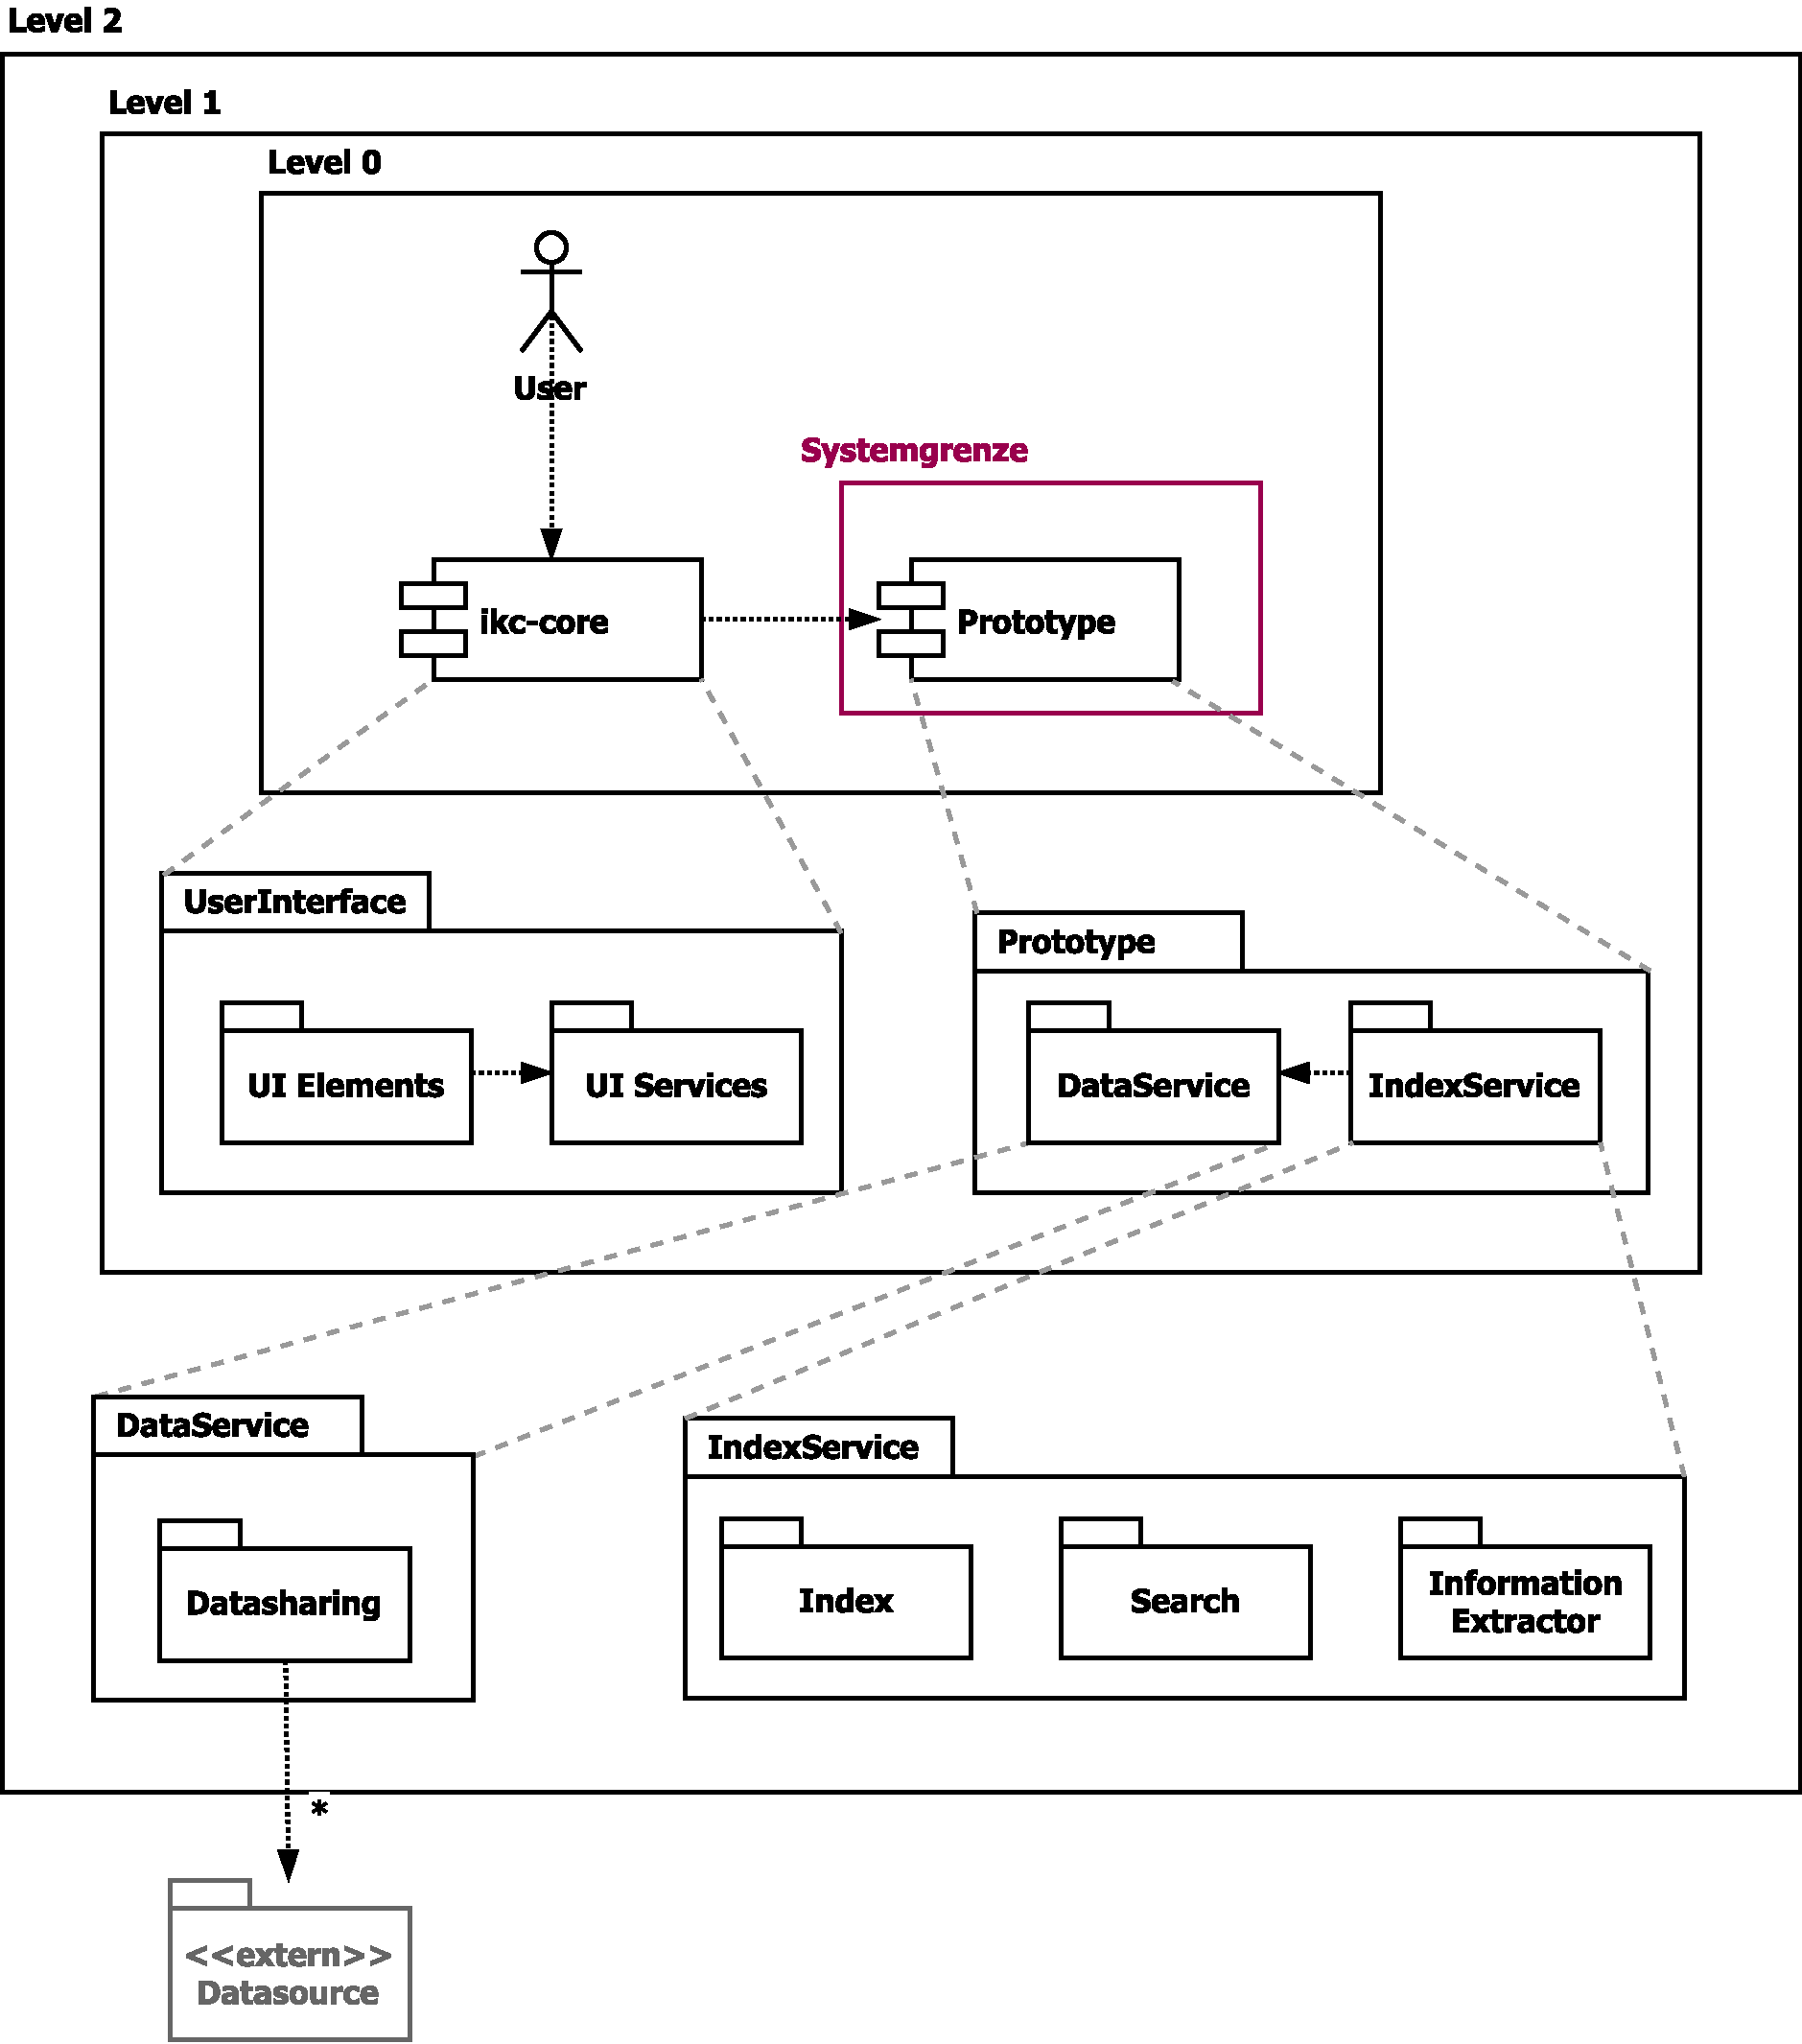
\includegraphics[width=1\textwidth]{BDA_Whitebox}
\caption{Bausteinsicht}
\label{fig:bausteinsicht}
\end{figure}

Nachfolgend werden diese näher erläutert.

\subsubsection{Bausteinsicht Level 0}
Innerhalb des \texttt{Level 0} werden die Zusammenhänge zwischen dem \texttt{User}, dem \texttt{ikc-core} und dem \texttt{Prototypen} aufgezeigt. Ebenfalls ist die Systemgrenze zwischen der bestehenden und der zu erstellenden Komponente ersichtlich. Die Systemgrenze grenzt den Kern des Prototyps ein.

\sssubsection{User}
Wie bisher hat der Benutzer über die Benutzeroberfläche des \gls{ikc-core} Zugriff auf alle Funktionalitäten. Die Zusatzfunktionen, welche durch den Prototyp zur Verfügung gestellt werden, sind für den Benutzer in der Suchfunktion und den extrahierten Schlüsselwörter ersichtlich.

\sssubsection{ikc-core}
Neben den bisherigen Funktionalitäten nutzt der \texttt{ikc-core} zusätzlich die neuen Funktionen, welche vom Prototypen zu Verfügung gestellt werden. Dazu zählt die Volltextsuche und die Schlüs\-sel\-wort-\-Ex\-trak\-tion. Er besteht prinzipiell aus verschiedenen \texttt{UI\-Ele\-ments} welche \texttt{UI\-Ser\-vices} nutzen um zugrundeliegende Logik zu kapseln. In dieser Logik soll der \texttt{Prototype} integriert werden.

\sssubsection{Prototype}
Die Komponente \texttt{Prototype} kapselt die essentiellen Funktionen, die Textanalyse und die Anbindung der externen Datenquelle. Darin unterschiedenen werden die Module \texttt{DataService} und \texttt{IndexService}.

\sssubsection{Bausteinsicht Level 1}
Mithilfe des zweiten Abstraktionlevels (\texttt{Level 1}) werden die verschiedenen Module und die Beziehung innerhalb der Komponente aufgezeigt. 

\sssubsection{UI Elements}
Die Interaktion mit dem Benutzer wird durch die Komponente \texttt{UI\-Ele\-ments} abgehandelt. Dabei werden alle sichtbaren Teile der Oberfläche in verschiedene Elemente gekapselt. Die resultierenden Elemente sollen innerhalb der Applikation beliebig wiederverwendbar sein (zum Beispiel \texttt{SearchField}). Mit Hilfe des Applikationzustandes wird der Inhalt der Elemente festgelegt.

\sssubsection{UI Services}
Die Logik der Applikation wird in verschiedene \texttt{UIServices} aufgeteilt, diese steuern das Verhalten der Applikation durch die Aktualisierung des jeweiligen Applikationzustandes.

\sssubsection{DataService}
Das Modul \texttt{DataService} regelt den Zugriff auf externe Datenquellen. Dank der Abstraktion des spezifischen Zugriffs können verschiedene Quellen, je nach Bedarf, verwendet werden. Weiter kann der Zugriff mittels der Freigabe-Token an andere Module weitergegeben werden. %Weiter soll es anderen Modulen der Applikation, mithilfe von Freigabe-Token, Elemente der externen Datenquelle freigegeben werden.

Diagramm

Innerhalb der Komponente der Bachelorarbeit beschränkt man sich auf die Verwendung von externen Datenquellen über \gls{SFTP}. Eine Erweiterung verschiedener Datenquellen soll jedoch möglich sein.

\sssubsection{IndexService}
Die eigentliche Textanalyse wird mit dem Modul \texttt{IndexService} durch\-ge\-führt. Die beiden Teilmodule \texttt{Search} und \texttt{InformationExtraction} nutzen den \texttt{Index} als Basis für die Berechnung von Suchresultaten oder die Extraktion von Schlüsselwörtern.

\subsubsection{Bausteinsicht Level 2}
Mit Hilfe des letzten Abstraktionslevels (\texttt{Leve 2}) der Bausteinsicht werden die verschiedenen Teilmodule erläutert.

\sssubsection{DataAccess}
Eine der Hauptaufgaben des \texttt{DataService}-Moduls, der Zugriff auf verschiedene externe Datenquellen, wird mittels des Teilmoduls \texttt{Data\-Sharing} abgehandelt. Darin wird der spezifische Zugriff auf die Quelle beschrieben.

\sssubsection{DataSharing}
Neben dem Zugriff sollen Elemente von externen Quellen innerhalb der Applikation via Freigabe-Token zu Verfügung gestellt werden. Diese werden innerhalb des \texttt{DataSharing} Teil-Moduls gehalten. Nach einmaliger Verwendung sollen diese verfallen.

\sssubsection{Datasource}
Über das externe Modul \texttt{DataSource} findet der Zugriff auf externe Datenquellen statt. Einerseits können hier Daten im Volltext bezogen werden, andererseits können hier Konfigurationsdaten oder Indizes gespeichert werden.

\sssubsection{Index}
Innerhalb des Teilmoduls \texttt{Index} wird der Text-Korpus zusammen mit allen wichtigen Informationen gehalten. Dazu gehört insbesondere der Volltext-Index für die Suche, als auch Informationen zu der Anzahl der Vorkommnisse potentieller Schlüsselwörter innerhalb des Korpus. Er bildet somit die Grundlage für die Volltextsuche und die Schlüsselwortextraktion.

\sssubsection{Search}
Das Teil-Module \texttt{Search} handelt Suchanfragen ab. Die Resultate werden basierend auf dem Volltext Index generiert. 

\sssubsection{InformationExtractor}
Die Extraktion von Schlüsselwörter wird durch das Teil-Modul \texttt{In\-for\-ma\-tion\-Ex\-trac\-tor} angehandelt. Basierend auf dem \texttt{Index} berechnet er eine Auswahl aus den potentiellen Kandidaten.

\newpage

\subsection{Ablaufsicht}

Die \autoref{fig:ablaufsicht} gewährt einen Überblick über den Gesamtablauf vom Beginn der Nutzung des \gls{ikc-core} bis zum Betrachten der Suchresultate oder der extrahierten Schlüsselwörter. 

Der Benutzer ist Ursprung der Abläufe: Er nutzt den \gls{ikc-core} und hat darin eine externe Datenquelle (beispielsweise \gls{SFTP}) hinterlegt. Sind diese Voraussetzungen erfüllt, holt sich der \gls{ikc-core} beim \texttt{Da\-ta\-Ser\-vice} die Freigabe für die benötigten Daten (\texttt{shareData}). Benötigte Daten können die berechneten Indizes oder den Volltext der Dateien beinhalten. Der \texttt{DataService} antwortet und gibt damit die Freigabe zurück. 

\begin{figure}[h]
\centering
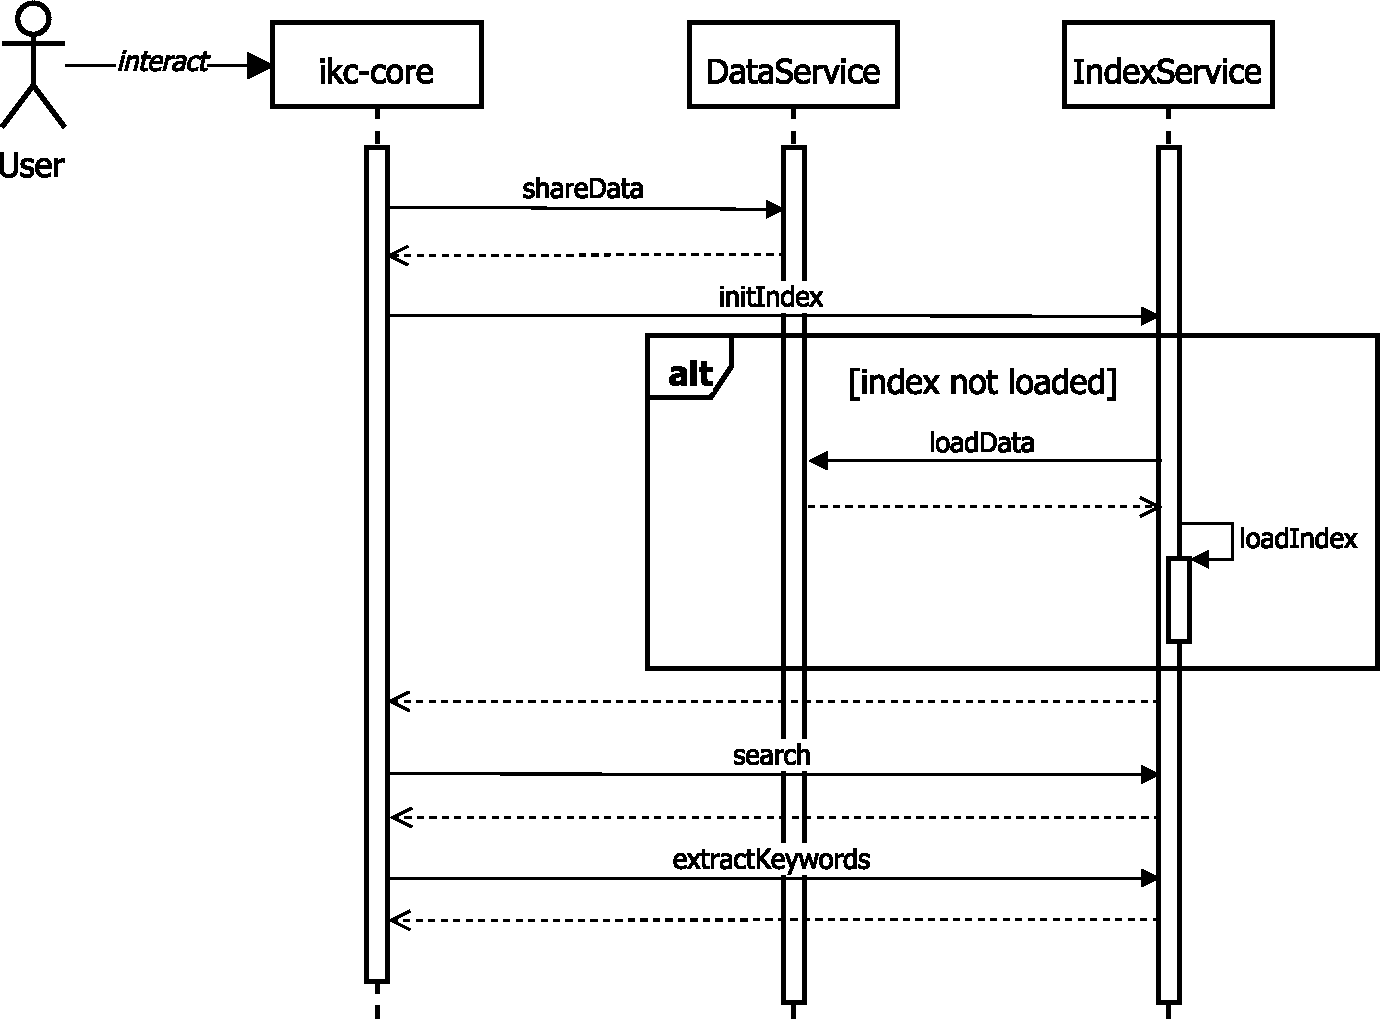
\includegraphics[width=1\textwidth]{BDA_Sequence}
\caption{Ablaufsicht}
\label{fig:ablaufsicht}
\end{figure}

Die erhaltene Freigabe gibt der \gls{ikc-core} im Prozess \texttt{initIndex} an den \texttt{IndexService} weiter. Hat dieser den angeforderten Index bereits geladen, gibt er diesen an den \gls{ikc-core} zurück. Ist dies nicht der Fall, holt er sich beim \texttt{Data\-Service} wiederum die benötigten Daten (\texttt{loadData}). Diese können denselben Inhalt wie oben haben. Das ist abhängig davon, ob er Index bereits erstellt wurde. Falls nicht, muss dieser auf Basis aller Dateien erstellt werden. Ist er bereits erstellt oder nach dessen Erstellung wird dies an den \gls{ikc-core} gemeldet.

Nun kann der \gls{ikc-core} die Funktionalität des \texttt{IndexService} nutzen: Er hat Zugriff auf die Volltextsuche (\texttt{search}) und die extrahierten Schlüsselwörter (\texttt{extractKeywords}). 

\subsection{Verteilung}

Wie oben schon angesprochen, findet die Entwicklung sowohl client- als auch serverseitig statt. \autoref{fig:verteilung} gibt einer detaillierten Üb\-er\-blick. Auf der Seite des Clients läuft der \gls{ikc-core} im Browser. Dieser verwendet für die Zwischenspeicherung von Daten eine \gls{in-browser Datenbank}

    
        \begin{figure}[H]
    \centering
    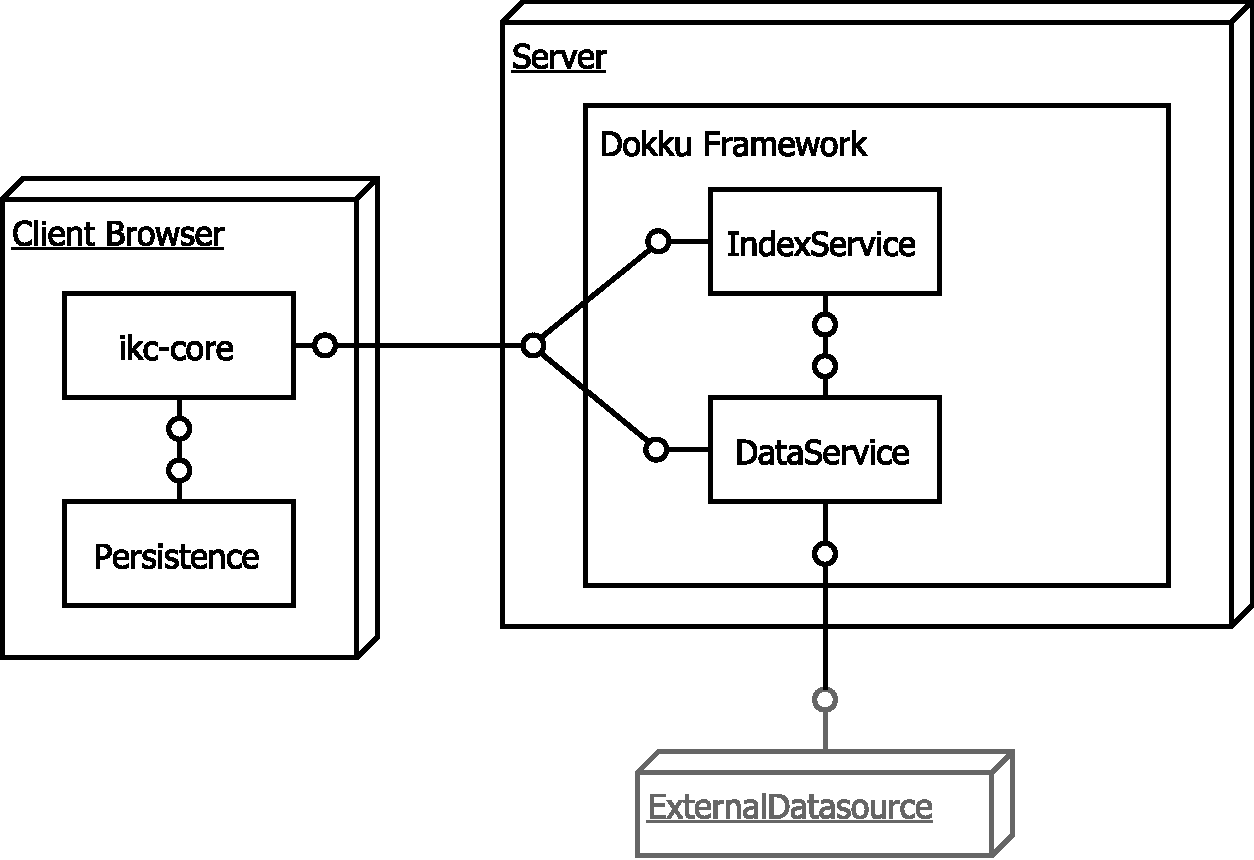
\includegraphics[width=0.7\textwidth]{DistributionView}
    \caption{Verteilung}
    \label{fig:verteilung}
    \end{figure}

% ----------------------------------------------------------------


\section{Algorithmus}
Der Kern des Prototypen bilden die verschiedene Algorithmen. Basierend auf den externen Datenquellen ermöglichen sie eine Volltext-Suche und die Extraktion der relevanten \gls{Keyword}[s]. Nachfolgend werden die Funktionsweise als auch wichtigsten Überlegungen dazu veranschaulicht. Basierend auf verschiedenen bestehenden Ansätzen wird die Lösungsfindung für den hier verwendeten Algorithmus dargelegt. 


Um die relevanten \gls{Keyword}[s] für ein spezifisches Dokument zu extrahieren werden verschiedenen Methoden aus dem Feld von \hyperref[natural-language-processing]{\textit{Natural Language Processing}} kombiniert mit statistischen Analsysen und heuristischen Vorgaben. Für die Analyse der \gls{Keyword}[s] werden \gls{N-Gramm}[e] der grösse eins bis vier berücksichtigt. Nebst möglichst treffenden Resultaten liegt der Fokus auch auf der raschen Aussortierung von ungeeigneten Kandidaten. Da die Berchnung der Relvanz der Rechen- und Speicher-Intensivste Vorgang des Algorithmus ist.  Die Anzahl mögliche \gls{N-Gramm}[en] ist definiert als: 
\[f(x)=\sum_{n=0}^N x - n  
\begin{cases} 
   (x - n)  & \text{if } x > n \\
   0      & \text{if } x \leq n
  \end{cases}\]
Wobei $N$ die maximale Länge eines \gls{N-Gramm} und $x$ die Länge des Textes representieren.

In der \autoref{fig:seq_keywordextraction} wird dafür Konzeptionelle Ablauf graphisch dargestellt und anschliessend die verschiedenen Elemente genauer erläutert.

    \begin{figure}[H]
    \centering
    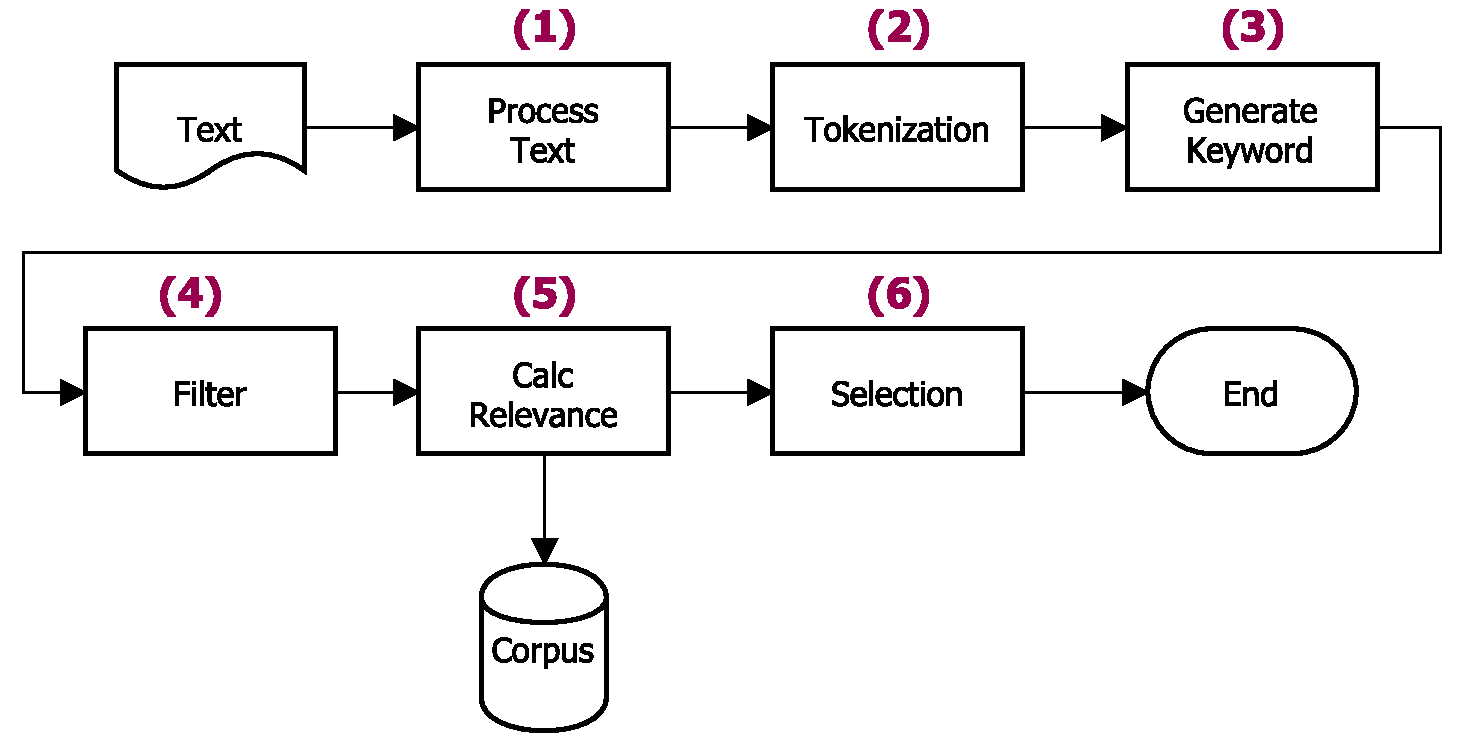
\includegraphics[width=1\textwidth]{KeywordExtraction}
    \caption{Ablauf Schlüsselwort-Extraktion}
    \label{fig:seq_keywordextraction}
    \end{figure}
 

\subsection{Eingabe}
Als Eingabe in den Algorithmus wird eine Text erwartet. Im Fall dieses Prototypen handelt es sich ein Wikipedia Artikel aus den Trainings Daten. Um die verschiedenen folgenden Schritt besser zu illustrieren, wird der folgende Satz als Beispiel Text verwendete. Mit einer Länge von $19$ Wörter, besitzt er $70$ mögliche \gls{N-Gramm}[e] mit Länge eins bis vier.

\begin{quote}
\textit{The Guardian newspaper was founded in 1821 as \glqq The Manchester Guardian\grqq, which head office is still located in Manchester.}
\end{quote}
Mit einer Länge von $19$ Wörter, besitzt er $70$ mögliche \gls{N-Gramm}[e] mit Länge eins bis vier.

\subsection{(1) Vorverarbeitung}
Im ersten Schritt wird der Text anhand verschiedener Vorgaben vorbereitet. Dazu werden zu Beginn nach einem Punkt, einem Fragezeichen, Ausrufezeichen oder einem Zeilenschaltung, der nachfolgende Buchstaben in die Kleinschreibung umgewandelt. Dies dient dazu Wörter zu erkennen, welche als Nomen genutzt werden jedoch nicht aus diese Wortart stammen. Dadurch verändert sich der Beispiel Satz geringfügig. 

\begin{quote}
\textit{\textbf{t}he Guardian newspaper was founded in 1821 as \glqq The Manchester Guardian\grqq, which head office is still located in Manchester.}
\end{quote}

Weiter wird nun der Text in Fragmente aufgeteilt. Dabei wird davon ausgegangen, dass sich relevante \gls{Keyword}[s] nicht über eine Satzzeichen erstrecken. Es entsteht eine Abfolge von Text Fragmenten.
\begin{quote}
\textit{\textbf{(}the Guardian newspaper was founded in 1821 as\textbf{)} \textbf{(}The Manchester Guardian\textbf{)} \textbf{(}which head office is still located in Manchester\textbf{)}}
\end{quote}
Nach dem ersten Schritt wurde der Text mit $19+18+17+16=70$ möglichen \gls{N-Gramm}[en] in eine List von Text-Fragmente mit $(8+7+6+5)+(3+2+1)+(8+7+6+5)=58$ möglichen \gls{N-Gramm}[en] transformiert. Dadurch konnten bereis $12$ Kandidaten ausgeschlossen werden.


\subsection{(2) Text zerlegung}
Bevor die eigendliche Kandidaten gebildetet werden, werden nun die Text-Fragmente durch das \hyperref[tokenization]{\textit{Tokenization}} aufgeteilt in eine List von einzelnen Wörter. Ebenfalls werden dabei unerwünscht Sonderzeichen am Anfang oder am Ende eines Wortes entfernt. Dabei handelt es sich in erster Linie um alle anderen Satzzeichen welche bei der Aufteilung des Textes in Text-Fragmente nicht berücksichtigt wurden.

\begin{quote}
\textit{\textbf{[}the, Guardian, newspaper, was, founded, in, 1821, as\textbf{]}, \textbf{[}The, Manchester, Guardian\textbf{]}, \textbf{[}which, head, office, is, still, located, in, Manchester\textbf{]}}
\end{quote}

\subsection{(3) Generierung möglicher Keywords}
Anhand der generierten Wort Listen können nun die verschiedenen \gls{N-Gramm}[e] generiert werden. Es entsteht eine List von \gls{N-Gramm}[en] der Länge von eins bis vier.

\begin{quote}
\textit{\textbf{[}the Guardian newspaper was, the Guardian newspaper, the Guardian, the, ... , located in Manchester, located in, located, in Manchester, in, Manchester\textbf{]}}
\end{quote}

\subsection{(4) Filter mittels POS-Tagger}
Wie von \cite{parameswaran2010towards} beschrieben folgen Relevante \gls{Keyword}[s] bestimmten grammatikalischen Regeln. Diese sind wie folgt definiert:
\begin{enumerate}
    \item Ein relevantes \gls{Keyword} besteht mindestens aus einem Nomen. Somit werden entfallen \gls{Keyword}[s] wie zum Beispiel \textit{was} oder \textit{located in}.
    \item Ein relevantes \gls{Keyword} beginnt nicht mit einem Pronomen, Verb oder Partikel. Diese Regel ist in der Lage \gls{Keyword}[s] wie \textit{the Guardian newspaper} auszusortieren.
    \item Ein relevantes \gls{Keyword} endet nicht mit einem Pronomen, Verb oder Partikel. Diese Regel ist in der Lage \gls{Keyword}[s] wie \textit{Guardian newspaper was} auszusortieren.
\end{enumerate}
Wie bereits erwähnt möchten auch Nicht-Nomen welche als solche verwendetet werden berücksichtigt werden. Dafür werden die zwei Regeln mit einer dritten erweitert:
\begin{enumerate}
    \item[4.] Ein relevantes \gls{Keyword} beginnt gross. Wie bereits erwähnt wurden vor gängig innerhalb des Textes Wörter nach bestimmten Satzzeichen in die Kleinschreibung umgewandelt, damit diese in diesem Schritt nicht beachtet werden. Dadurch wird zum Beispiel \textit{The Manchester Guardian} weiter beachtet auch wenn er grundsätzlich der zweiten Regel widerspricht da er mit einem Pronomon startet. 
\end{enumerate}
Um diese Regeln zu Überprüfen wird ein \hyperref[part-of-speech]{Part-Of-Speech-Tagger} verwendet. Dabei handelt es sich um Algorithmus mit welchem die Worarten von gegebenen Wörter bestimmt werden kann. Um den Regeln zu entsprechen muss ein \gls{Keyword} sowohl Regeln 1\&3 folgend, zusätzlich entweder der Regel 2, Regel 4 oder beiden. Mittels dieser drei Regeln können alle möglichen Kandidaten ausser den folgenden ignoriert werden:

\begin{quote}
\textit{\textbf{[}Guardian newspaper, Guardian, newspaper, 1821, The Manchester Guardian, The Manchester, The, Manchester Guardian, Manchester, Guardian, head office, head, office, Manchester\textbf{]}}
\end{quote}

Damit sind noch $14$ mögliche \gls{Keyword}[s] von ursprünglich $70$. Anschliessend werden gleiche \gls{Keyword}[s] zusammengfasst indem sie zusammen mit ihrer Anzahl Vorkomnisse kombiniert werden, somit reduziert sich die Anzahl unterschiedlichen \gls{Keyword}[s] auf $12$ (\autoref{keyword-with-count}). Ebenfalls wird jeweils das erste Wort eines \gls{Keyword}[s] kleingeschrieben falls es sich nicht um ein Nomen handelt. So kann sichergestellt werden, dass zum Beispiel das 1-Gramm "The" im nächsten Schritt tiefer gewertet wird. Da die Grosschreibung nur im Kontext des \gls{Keyword}[s] \textit{The Manchester Guardian} von Bedeutung ist.

\begin{longtable}{|p{4cm}| p{1cm}|}
  \hline
    \gls{Keyword} & \#\\\hline
    Guardian & 2  \\\hline
    Manchester & 2  \\\hline
    Guardian newspaper & 1  \\\hline
    newspaper & 1  \\\hline
    1821 & 1  \\\hline
    the Manchester Guardian & 1  \\\hline
    the Manchester & 1  \\\hline
    the & 1  \\\hline
    Manchester Guardian & 1  \\\hline
    head office & 1  \\\hline
    head & 1  \\\hline
    office & 1  \\\hline
        \caption{Keyword mit Vorkomniss}
    \label{keyword-with-count}
\end{longtable}

\subsection{(5) Berechnung der Relevanz}\label{calcrelevance}
Um die verschiedenen \gls{Keyword}[s] zu gewichten wird ein individueller Score pro \gls{Keyword} ausgerechnent. Dazu werden folgende Metriken benötigt (\autoref{metric-per-keyword}).

\begin{longtable}{|p{2cm}| p{8cm}|}
  \hline
    Metrik & Erläuterung\\\hline
    $numDocs$ & Anzahl Dokument im Korpus  \\\hline
    $docFreq$ & Anzahl Dokument im Korpus welche diese \gls{Keyword}[s] enthalten  \\\hline
    $docLength$ & Anzahl Wörter des spezifischen Dokumentes \\\hline
    $freq$ & Haufigkeit des \gls{Keyword}[s] innerhalb des Dokuments. \\\hline
    \caption{Benötigte Metriken}
    \label{metric-per-keyword}
\end{longtable}


Basierend auf den eingeführten Metriken wird mit Hilfe einer angepassten Version der \textit{Similarity}-Formel\footnotemark \footnotetext{\cite{TFIDFSim65:online}} des \textit{Apache Lucene} Projekts den jeweiligen Score berechnet.

\begin{equation}\label{tf}
tf = \sqrt{freq} 
\end{equation}
\begin{equation}\label{idf}
idf  =  1 +log( \frac{numDocs}{1 + docFreq})
\end{equation}
\begin{equation}\label{lengthNorm}
lengthNorm =\frac{1}{\sqrt[3]{docLength}} 
\end{equation}
\begin{equation}\label{tfidf}
tfidf = tf * idf^2 * lengthNorm
\end{equation}

\autoref{tf} repräsentiert die Häufigkeit des \gls{Keyword}[s] innerhalb des gegebenen Dokument. Wenn die Anzahl steigt so steigt auch der \textit{tf}-Wert. Um die Empfindlichkeit zu reduzieren, wird der Wert gedämpft mittels der Wurzel-Funktion. 

Neben der Häufigkeit innerhalb des Dokuments ist die inverse Häu\-fig\-keit (\autoref{idf}) ein wichtiger Wert. Dadurch wird die Einzigartigkeit des \gls{Keyword}[s] innerhalb des Korpus ausgedrückt. Dieser Wert sinkt je öfter das gleiche \gls{Keyword} in andere Dokumente enthalten ist. Mittels der Addition von $1$ im Nenner innerhalb der Logarithmus Funktion wird eine Division durch Null verhindert. 

Würde mittels der \autoref{tf} \& \autoref{idf} der Score berechnet werden, so würden kurz und lange Dokumente Werte in andere Bereichen produzieren. Eine Verwendungen eines Schwellwerte für Begrenzung der \gls{Keyword}[s] wäre unmöglich. Dazu wird der Wert mit Hilfe der Dokumenten-Länge normalisiert. Dazu wird mittels der \autoref{lengthNorm} der Score normalisiert

\subsection{(6) Auswahl}
Schlussendlich werden die berechneten \gls{Keyword}[s] mithilfe eines Schw\-el\-werts begrenzt, somit wird eine Sinnvolle Anzahl an Dokumenten zurückgegeben. Im Gegensatz zu einer Limitierung der Anzahl \gls{Keyword}[s] kann mit einem Schwellwert je nach Text eine Anzahl an \gls{Keyword}[s] zurückgegeben werden, welche für den Text ideal ist.

\subsection{Dokumente für Schlüsselwort}
Die Gegenteilige Operation der \gls{Keyword} Extraktion ist Extraktion aller Dokument für ein bestimmtes  \gls{Keyword}. Dabei wird eine List an Dokumente erwartet, in welche ein bestimmtes \gls{Keyword} einen Höhen Score ausweisen kann. 

    \begin{figure}[H]
    \centering
    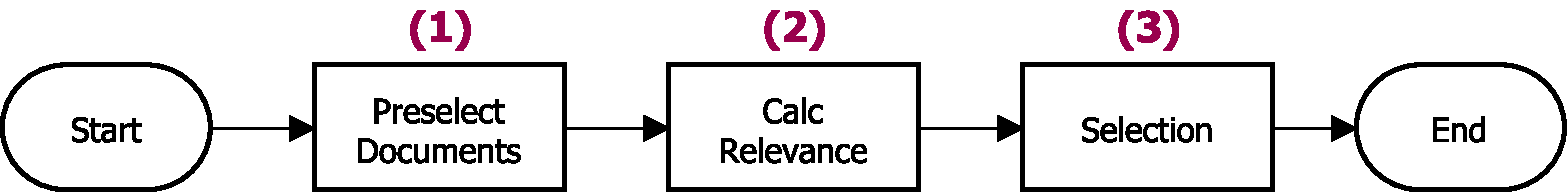
\includegraphics[width=1\textwidth]{DocumentForKeyword}
    \caption{Ablauf Relevante Dokumente für Schlüsselwort}
    \label{fig:seqdocforkeyword}
    \end{figure}
\begin{enumerate}
    \item  Dazu werden in einem ersten Schritt alle möglichen Dokumente ausgewählt. In dieser Menge an Dokumenten kommt das entsprechenden \gls{Keyword} mindestens einmal vor. Jedoch ungeachtet der Relvanz des \gls{Keyword}[s] für das jeweilige Dokument.
    \item In einem nächsten Schritt wird für jedes Dokument den jeweiligen Score für das bestimmte \gls{Keyword} berechnent. Die Berechnung folgt dabei exakt der bereits gesehenen Berchnungen der Relevanz (\autoref{calcrelevance}).

    \item Nun werden ebenfalls die Anzahl an Resultate mit Hilfe eines Schwellwerts reduziert. Somit kann die Auswahl auf die wirklich Relevantet Dokumente für das entsprechende \gls{Keyword} vermindert werden.
            
\end{enumerate}







% ----------------------------------------------------------------

\section{Integration des Prototypen}
Basierend auf der ausgeführten Architektur (\autoref{architecture}) werden im folgenden Abschnitt die wichtigsten Software-Konzepte erläutert. Dazu werden als erstes die grundlegenden Algorithmen ausgeführt. In einem zweiten Schritt wird deren Integration in den Prototypen dargelegt.

Im Gegensatz zum Architektur-Entwurf befasst sich der Software-Entwurf neben den tatsächlich verwendeten Software-Lösungen auch mit der Recherche nach geeigneten Möglichkeiten.

\subsection{Übersicht}


Im Klassendiagramm auf \autoref{fig:prototypeClassDiagram-easy} sieht man einen Überblick über den zu entwickelnden Prototypen. Abgebildet sind die wichtigsten Klassen und deren Beziehungen untereinander. Zunächst liegen die beiden Teile \gls{ikc-core} und \texttt{Prototype} vor. Der \gls{ikc-core} ist der aus dem Forschungsprojekt \gls{IKC} herausgehende bestehende Prototyp. Dieser nimmt Gebrauch von den beiden vom \texttt{Prototypen} zur Verfügung gestellten Schnittstellen des \texttt{Index-} und des \texttt{DataServices}.

Grundsätzlich besteht der \texttt{Prototyp} aus den zwei Komponenten \texttt{Index-} und des \texttt{DataService}. Diese verwenden die von ausserhalb ver\-füg\-bar\-en Models, das \texttt{In\-dex-} und das \texttt{DataModel}. Diese enthalten die Protokolle für die jeweilige Kommunikation, werden somit auch vom \gls{ikc-core} in Anspruch genommen.

Im der Implementation \texttt{Index-} beziehungsweise \texttt{DataServices}.

    \begin{figure}[H]
    \centering
    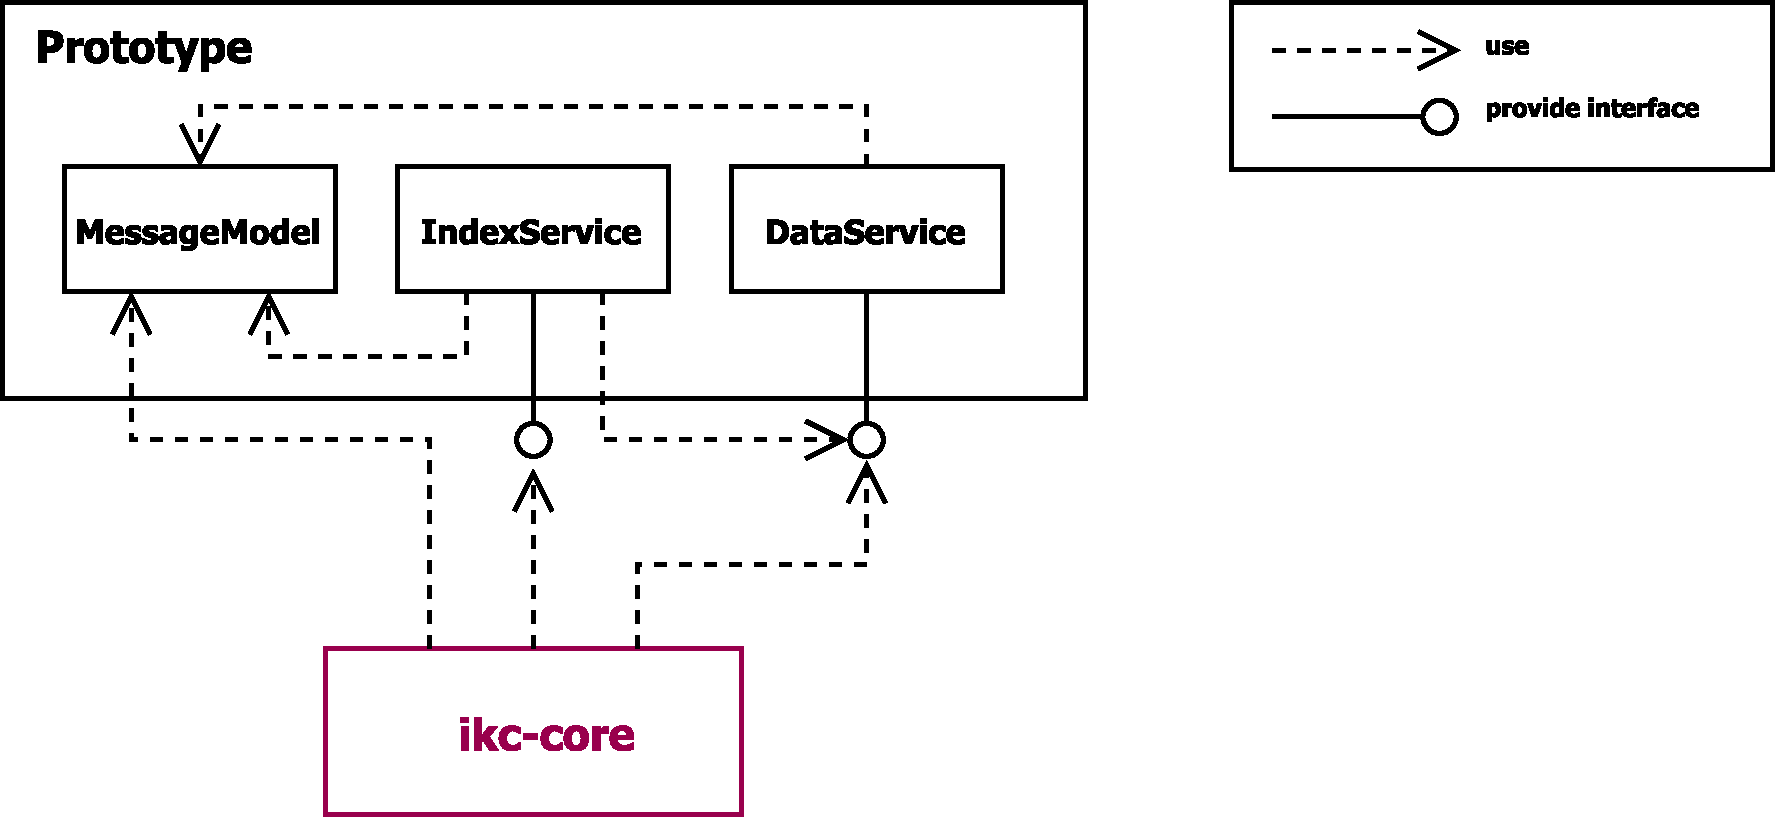
\includegraphics[width=1\textwidth]{ClassDiagrammGeneral}
    \caption{Prototype Klassendiagram}
    \label{fig:prototypeClassDiagram-easy}
    \end{figure}

Der Kern der Software bildet der Algorithmus, dieser ist, neben der Suchfunktionalität und dem Aufbau der Indizes, ein Hauptbestandteil des \texttt{IndexService}. \autoref{fig:kommunikation} gewährt einen Überblick über die beteiligten Komponenten. Als Grundlage benötigt der \texttt{In\-dex\-Ser\-vice} alle zu indexierenden Dateien im Volltext. Deren Quelle ist der \texttt{Data\-Ser\-vice}. Der \texttt{Index-} und der \texttt{DataService} bilden zusammen den eigentlichen Prototypen. Wie in der Bausteinsicht auf \autoref{fig:bausteinsicht} zu erkennen, gibt es neben der Integration der Services auch eine Einbindung in die bestehende Benutzeroberfläche des \gls{ikc-core}.


\subsection{Schnittstellen}
Der Prototyp soll sich möglichst nahtlos in den \gls{ikc-core} integrieren. Um dies zu erreichen sollen in keiner Situation Funktionen des \gls{ikc-core} blockiert werden durch den Prototypen. 

So werden Suchresultate des Index innerhalb der bestehenden Suche integriert und bei Bedarf aktualisiert. Die verschieden Resultate der verschiedenen Quellen sollen in Echtzeit nach ihrem Eintreffen dargestellt werden. Somit wird sich die Liste mit Resultate trotz gleichem Suchbegriff über die Zeit verändern, da weitere Resultate von entfernten Quellen eintreffen. 

Weiter sollen extrahierte \gls{Keyword}[s] klar getrennt von den bestehenden Properties des Nodes als \textit{Chips} oberhalb des Titel dargestellt werden. Sowohl ein Dokument mit entsprechenden \gls{Keyword}[s] als auch eine \gls{Keyword} mit den verknüpften Dokumenten werden als Node dargestellt. \autoref{fig:bda_ui} zeigt einen Entwurf dieser Integration. 

    \begin{figure}[H]
    \centering
    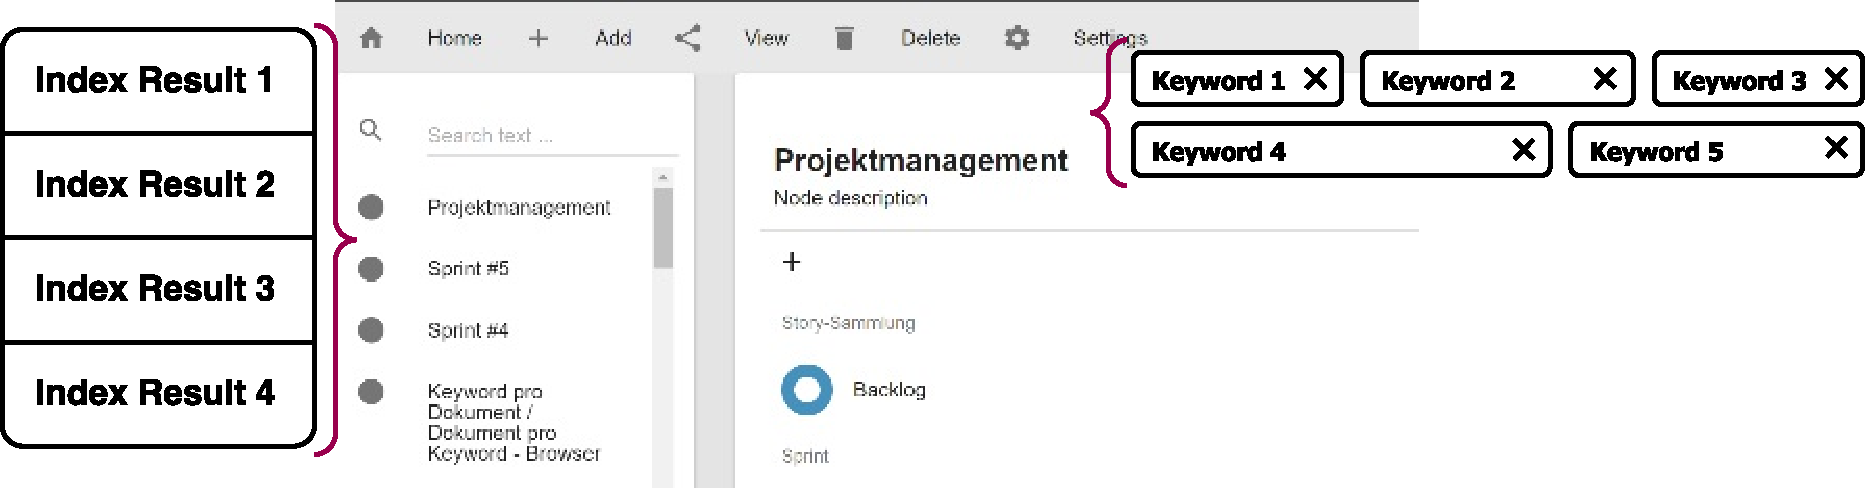
\includegraphics[width=1\textwidth]{BDA_UI}
    \caption{Entwurf Intgeration Benutzeroberfläche}
    \label{fig:bda_ui}
    \end{figure}

Um die Schnittstellen des Prototype ideal zu verwenden und die obigen Oberflächenanpassungen umzusetzten, sind Anpassungen bzw. Erweiterungen in der Software Struktur des \gls{ikc-core} nötig. Das Klassendiagramm (\autoref{fig:classDiagrammIkcCore-easy}) erläutert die wichstigsten Anpassungen:

%riesiges index.json, ungefähr 100k Files als Text-Dateien

\section{Datenfreigabe}
Für den Auftraggeber ist eine sichere Kommunikation. stetige Transparenz und Kontrolle über den Verbleib von benutzergenerierten Daten von hoher Wichtigkeit. Um diesen Anforderungen gerecht zu werden, wurde unter anderem ein Datenfreigabe-Konzept entwickelt. Dieses basiert auf \gls{Token}[s]. 






%ablaufdiagramm Einwegtoken Entkopplung

    \begin{figure}[H]
    \centering
    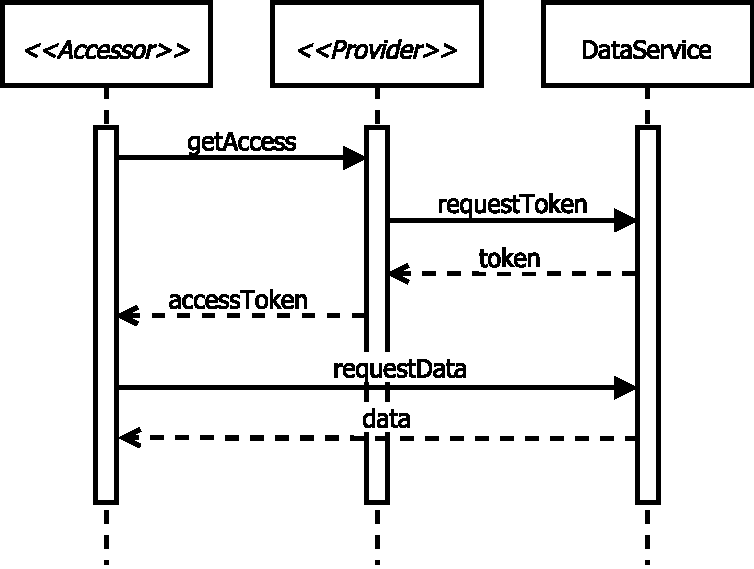
\includegraphics[width=0.8\textwidth]{SeqAccessGeneral}
    \caption{Ablauf: Datenfreigabe}
    \label{fig:seqaccesssession-easy}
    \end{figure}



\section{Auto-Indexierung}
